\usepackage{xcolor}
\usepackage{afterpage}
\usepackage{pifont,mdframed}
\usepackage[bottom]{footmisc}
\usepackage{tikz}
\usepackage{tikz-qtree}

\makeatletter
\gdef\this@inputfilename{input}
\gdef\this@outputfilename{output}
\makeatother

\newcommand{\funcitem}[2]{\item[$\blacksquare$] \textbf{\large \textsf{Funzione} \texttt{#1}} \vspace{-0.3cm} \begin{center}\begin{tabularx}{\textwidth}{|c|X|} \hline #2 \hline \end{tabularx}\end{center}}

Tra le varie opere di Leonardo, l'affresco raffigurante l'Ultima Cena è considerato uno dei maggiori capolavori. Un amico di Luca sta svolgendo una ricerca approfondita con il compito di fornire una descrizione esaustiva e particolareggiata di queste meraviglie.

Analizzando l'affresco, ha già individuato $N$ ``zone di interesse'' (come quelle racchiuse tra ellissi nella figura sotto), descritte con interi da $1$ a $N$, e $M$ relazioni tra di esse (indicate in figura con delle linee). I motivi per definire una relazione tra due zone sono molti: potrebbero contenere due personaggi che si stanno guardando, oppure due aree dipinte con tecniche similiari oppure completamente opposte, e così via.

\begin{figure}[h]
  \begin{center}
        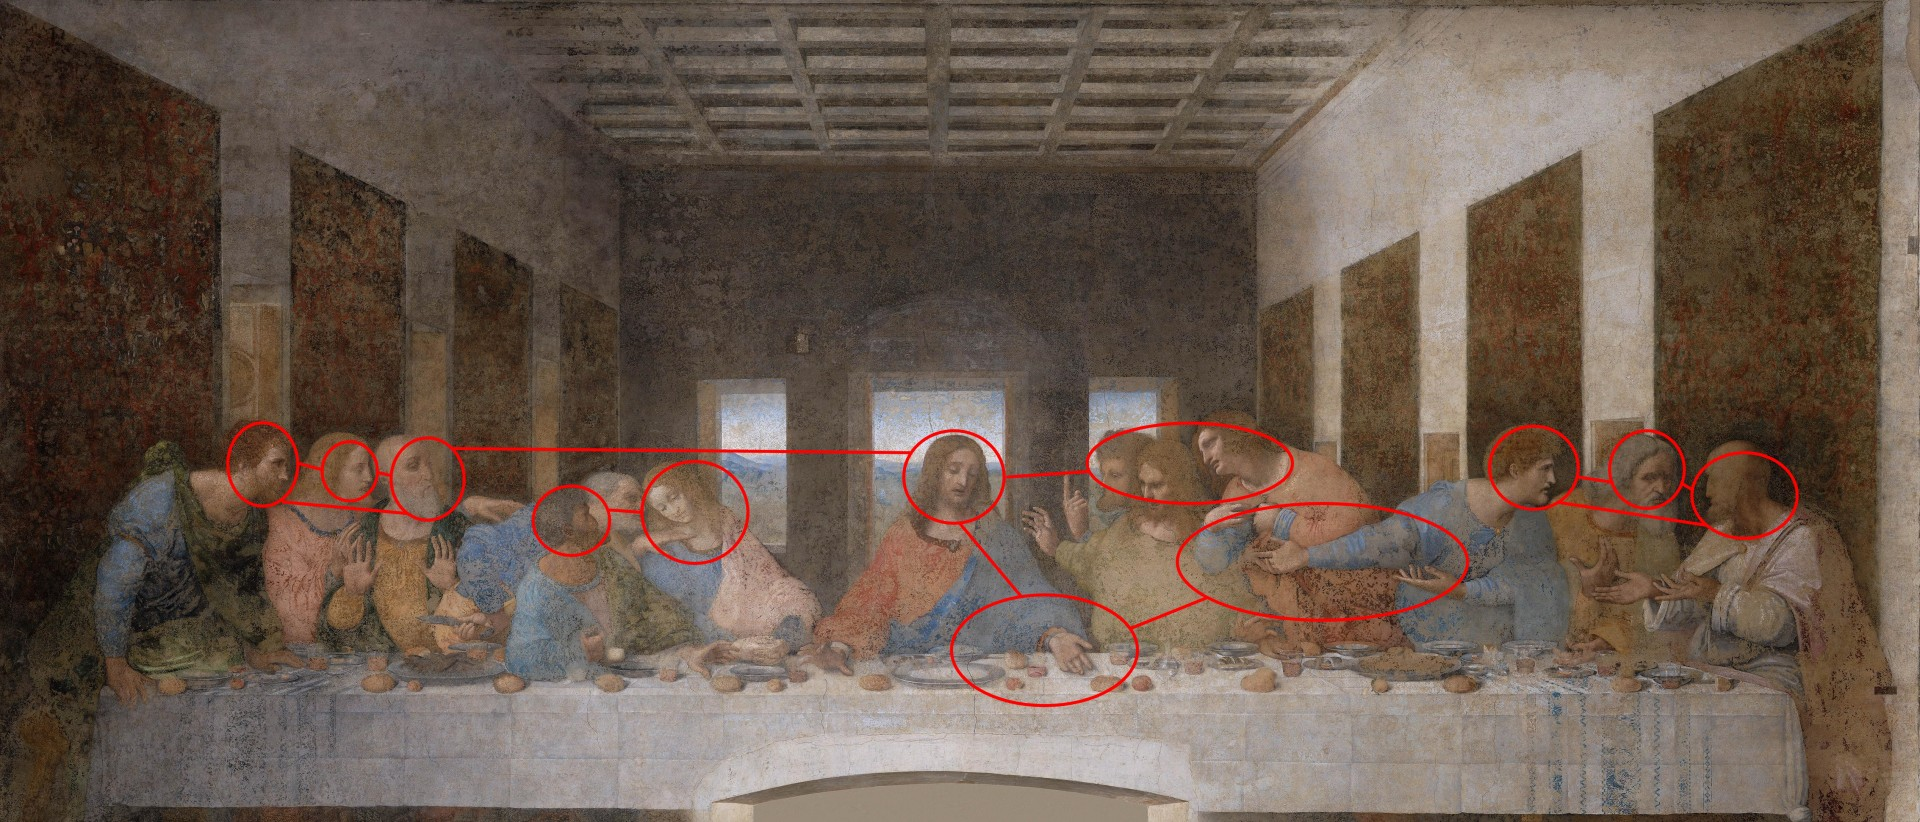
\includegraphics[width=\linewidth]{ultimacena.jpg}
        \caption{Cenacolo vinciano (annotato per evidenziare alcune delle zone di interesse e le loro relazioni).}
  \end{center}
\end{figure}

Il report finale del progetto di ricerca sarà costituito da un elenco delle zone di interesse. Per ognuna verranno descritte, oltre alla zona in sè, anche tutte le relazioni in cui è coinvolta.

Come suo solito, l'amico di Luca è stato particolarmente prolisso e ora il professore a capo del progetto di ricerca non vuole accettare il suo lavoro finché non farà una drastica selezione, includendo al più \textbf{dieci} zone di interesse.

Dopo tutto questo lavoro di accurata descrizione delle relazioni, l'amico è costretto a obbedire al professore ma non vuole sacrificare nemmeno una delle descrizioni già prodotte: aiutalo a selezionare un sottoinsieme $S$ delle $N$ zone in modo che il report finale contenga comunque la descrizione di \emph{tutte} le relazioni!


\Implementation
Dovrai sottoporre un unico file con estensione \texttt{.cpp} o \texttt{.c}.

\begin{warning}
Tra gli allegati a questo task troverai un template (\texttt{ultimacena.cpp} e \texttt{ultimacena.c}) con un esempio di implementazione.
\end{warning}

\pagebreak

Dovrai implementare la seguente funzione:

\begin{itemize}[nolistsep]
    \funcitem{riassumi}{
        C/C++  & \verb|int riassumi(int M, int M, int A[], int B[], int S[]);|\\
    }

    \begin{itemize}[nolistsep]
        \item L'intero $N$ rappresenta il numero delle zone di interesse.
        \item L'intero $M$ rappresenta il numero delle relazioni tra le zone.
        \item Gli array \texttt{A} e \texttt{B}, indicizzati da $0$ a $M-1$, contengono alla posizione $i$ la seguente informazione: esiste una relazione tra le zone \texttt{A[$i$]} e \texttt{B[$i$]}.
        \item La funzione dovrà restituire il numero $S$ di zone da includere nel report finale e riempire l'array \texttt{S} (nelle posizioni da $0$ a $S-1$) con gli identificativi di tali zone.

    \end{itemize}
\end{itemize}

Il grader chiamerà la funzione \texttt{riassumi} in accordo a quanto specificato di seguito.

% % % % % % % % % % % % % % % % % % % % % % % % % % % % % % % % % % % % % % % % % % %
% % % % % % % % % % % % % % % % % % % % % % % % % % % % % % % % % % % % % % % % % % %


\Grader
Allegata a questo problema è presente una versione semplificata del grader usato durante la correzione, che potete usare per testare le vostre soluzioni in locale. Il grader di esempio legge i dati da \texttt{stdin}, chiama la funzione che dovete implementare e scrive su \texttt{stdout}, secondo il seguente formato.

Il file di input è composto da $M+1$ righe, contenenti:
\begin{itemize}[nolistsep,itemsep=2mm]
    \item Riga $1$: gli interi $N$ e $M$, separati da uno spazio.
    \item Righe $2,\ldots, M+1$: i due interi \texttt{A[$i$]} e \texttt{B[$i$]} per $i = 0,\ldots, M-1$.
\end{itemize}

Il file di output è composto da due righe, contenenti:
\begin{itemize}[nolistsep,itemsep=2mm]
    \item Riga $1$: il valore $S$ restituito dalla funzione \texttt{riassumi}.
    \item Riga $2$: i valori contenuti nell'array \texttt{S} (posizioni da $0$ a $S-1$) così come modificato dalla funzione \texttt{riassumi}.
\end{itemize}

% % % % % % % % % % % % % % % % % % % % % % % % % % % % % % % % % % % % % % % % % % %
% % % % % % % % % % % % % % % % % % % % % % % % % % % % % % % % % % % % % % % % % % %

\Constraints

\begin{itemize}[nolistsep, itemsep=2mm]
\item $2 \le N \le 50\,000$.
\item $1 \le M \le 100\,000$.
\item È sempre garantita l'esistenza di una soluzione, ovvero esiste sempre un sottoinsieme costituito da al più dieci zone che rispetta quanto richiesto.
\item Se esistono più soluzioni è possibile stamparne una qualsiasi.
\item L'ordine con cui vengono riportate le zone in una soluzione è irrilevante.
\item Una relazione non viene mai ripetuta in input; inoltre $A_i \neq B_i$ per ogni $i = 0 \ldots M-1$.
\item Ogni zona d'interesse è coinvolta in almeno una relazione.
\end{itemize}

\Scoring
Il tuo programma verrà testato su diversi test case raggruppati in subtask.
Per ottenere il punteggio relativo ad un subtask, è necessario risolvere
correttamente tutti i test relativi ad esso.
\begin{itemize}[nolistsep,itemsep=2mm]
\item \textbf{\makebox[2cm][l]{Subtask 1} [\phantom{0}0 punti]}: Casi d'esempio.
\item \textbf{\makebox[2cm][l]{Subtask 2} [40 punti]}: $N \le 15$.
\item \textbf{\makebox[2cm][l]{Subtask 3} [40 punti]}: $N \le 1000$.
\item \textbf{\makebox[2cm][l]{Subtask 4} [20 punti]}: Nessuna limitazione specifica.
\end{itemize}

\Examples
\begin{example}
\exmpfile{ultimacena.input0.txt}{ultimacena.output0.txt}%
\exmpfile{ultimacena.input1.txt}{ultimacena.output1.txt}%
\end{example}

\Explanation

Nel \textbf{primo caso di esempio} le zone di interesse sono così poche da poter essere incluse tutte nel report senza problemi. Naturalmente sarebbe stato ammissibile produrre soluzioni diverse (ad esempio includendo le sole zone 3 e 4).


Nel \textbf{secondo caso di esempio} ci sono $11 > 10$ zone di interesse, quindi dobbiamo escluderne (almeno) una. Possiamo escludere la zona 1, le cui uniche relazioni sono con le zone 3 e 4 già incluse nel report finale.

\begin{solution}
    \renewcommand{\O}{\mathcal{O}}
\createsection{\Esponenziale}{{\small{$\blacksquare$}} \normalsize Soluzione esponenziale}
\createsection{\FPT}{{\small{$\blacksquare$}} \normalsize Vertex-cover è trattabile fissato il parametro (FPT)}
\createsection{\Osservazione}{{\small{$\blacksquare$}} \normalsize Un'ulteriore osservazione}

Questo problema è una versione mascherata del noto ``problema di copertura dei vertici'', forse più conosciuto con la dicitura inglese \emph{vertex-cover}.

Possiamo sintetizzare il problema come segue: dato un grafo $G=(V,E)$ si vuole trovare un sottoinsieme dei suoi vertici $S \subseteq V$ tale che ogni arco abbia almeno un estremo in $S$. In altre parole, per ogni $(u,v) \in E$ almeno un vertice tra $u$ e $v$ deve essere incluso nell'insieme $S$, che è detto \emph{copertura}.

Questo problema è \emph{NP-completo}, ovvero appartiene a una classe di problemi detta \emph{NP}, per i quali possiamo verificare se una soluzione è ammissibile in tempo polinomiale. Nel caso di vertex cover, quindi, dato un insieme di vertici è ``facile'' verificare se è davvero una copertura. Essendo inoltre anche un problema \emph{NP-hard}, si sospetta che per esso non esistano soluzioni polinomiali (a meno che \emph{P}$=$\emph{NP})\footnote{Ovviamente questa trattazione delle classi di complessità computazionale teoriche è solo una brevissima sintesi, ulteriori approfondimenti possono essere trovati facilmente nei libri classici di algoritmica oppure su Wikipedia}.

\Esponenziale
Abbiamo accennato che per i problemi \emph{NP} è ``facile'' verificare se la soluzione è corretta. Concentriamoci quindi ora sul nostro problema e descriviamo una semplice procedura che dato un insieme $S \subseteq V$, stabilisca se tale insieme è davvero una copertura valida per il grafo $G$. È sufficiente iterare su tutti gli elementi $s \in S$ e segnare come ``visitati'' tutti gli archi ad essi incidenti. Al termine, in tempo lineare nel numero dei vertici e degli archi, potremo affermare che $S$ è una copertura valida se e solo se tutti gli archi sono stati visitati.

Non resta altro che provare ``a forza bruta'' tutte le possibili combinazioni con cui è possibile formare insiemi di al più dieci elementi partendo dagli $N$ vertici del grafo. Uno dei modi più facili per implementare questa soluzione è far ricorso a una funzione ricorsiva che, richiamata via via su tutti i vertici, provi per ognuno ad includerlo oppure escluderlo dall'insieme candidato. Quando tale insieme raggiunge cardinalità dieci, si verifica se costituisce o meno una copertura tramite la procedura lineare descritta sopra.

Poiché le assunzioni garantiscono l'esistenza di tale copertura, esplorando tutte le possibilità siamo certi di trovarla, pagando purtroppo una complessità esponenziale.

\FPT
Con un po' di allenamento, ci si accorge che questo problema ha un'assunzione abbastanza singolare: qualunque sia la dimensione del grafo, esiste una copertura con al più dieci vertici. Questo da un lato può suggerire lo sviluppo di alcune euristiche greedy, sfruttando il fatto che i vertici nella copertura hanno probabilmente un alto numero di archi incidenti; dall'altro dovrebbe far riflettere sulla natura del problema.

Ribadiamo il fatto che siamo certi esista una copertura come richiesto. Preso allora un qualsiasi arco $(a,b)$ sicuramente $a$ deve appartenere alla copertura oppure $b$ deve appartenervi. Non può essere che la copertura non contenga né $a$ né $b$, perché altrimenti l'arco $(a,b)$ non sarebbe coperto, contro la definizione di copertura. Possiamo quindi ``esplorare'' due possibili casi: la copertura contiene $a$ oppure la copertura contiene $b$.

Proseguiamo allo stesso modo e consideriamo un arco $(b,c)$: se prima la scelta è ricaduta sull'includere $a$, ora possiamo includere $b$ oppure $c$ arrivando ad avere $\{a,b\}$ oppure $\{a,c\}$. Se invece prima avessimo scelto di includere $b$, ora l'arco $(b,c)$ sarebbe già coperto e non ci sarebbe bisogno di aggiungere nulla.

Consideriamo ancora un altro arco: $(d,e)$. A prescindere dalle scelte fatte in precedenza, abbiamo di nuovo due possibilità per coprirlo: aggiungere $d$ oppure $e$ alla copertura. Visualizziamo tramite un albero la situazione descritta.

	\begin{center}
		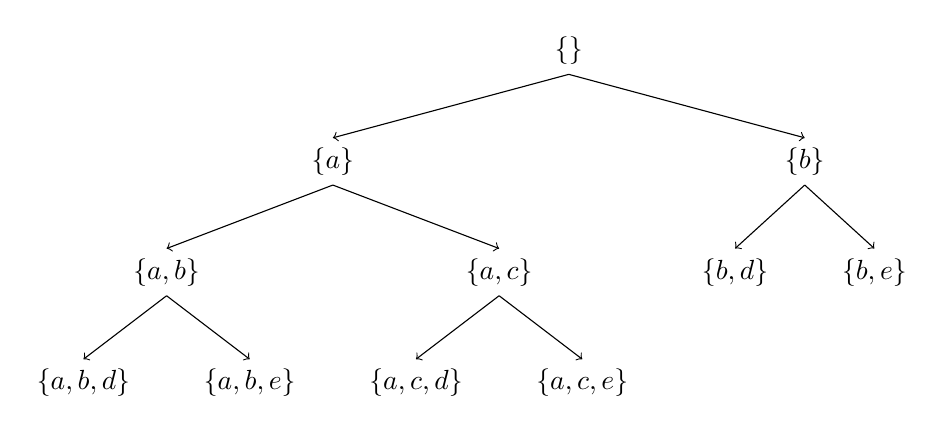
\begin{tikzpicture}
		\tikzset{level distance=40pt,sibling distance=20pt}
		\tikzset{edge from parent/.append style={->}}
                \Tree [.$\{\}$ [.$\{a\}$ [.$\{a,b\}$ [.$\{a,b,d\}$ ] [.$\{a,b,e\}$ ] ] [.$\{a,c\}$ [.$\{a,c,d\}$ ] [.$\{a,c,e\}$ ] ] ] [.$\{b\}$ [.$\{b,d\}$ ] [.$\{b,e\}$ ] ] ]
		\end{tikzpicture}
	\end{center}

Si può proseguire analizzando tutti gli archi e aggiungendo mano a mano le due possibilità (dove servono) per completare la copertura. Questa tecnica è detta \emph{bounded search tree}: stiamo costruendo un albero di ricerca della copertura, ma esso è limitato dalla dimensione massima della copertura. La chiave per non far espandere all'infinito l'albero e rischiare di percorrere strade non convenienti è proprio data dal limite dei dieci vertici. Questo particolare albero infatti è limitato a profondità dieci; se una foglia a profondità dieci non contiene ancora un insieme che copre tutto il grafo, non ha senso proseguire.

D'altra parte è relativamente facile convincersi che se una copertura esiste, con questo metodo sicuramente viene trovata entro profondità dieci perché stiamo analizzando tutti i possibili insiemi sensati (non aggiungendo inutilmente entrambi gli estermi di un arco) fino a dimensione dieci.

Questa categoria di problemi è detta \emph{FPT} (Fixed-Parameter Tractable): il problema generale è intrattabile, ma se imponiamo limiti sul ``parametro'' possiamo trovare una soluzione lineare nella dimensione dell'input ed esponenziale solo nel parametro. Nello specifico, per questo problema il parametro è la dimensione della copertura e la complessità della soluzione è $\O((N+M) \cdot 2^{10})$. Ciò non cancella i ragionamenti iniziali sull'intrattabilità del problema nella sua formulazione generale: stiamo semplicemente sfruttando un'assunzione importante sulla dimensione della soluzione del problema. 

\Osservazione
Per raggiungere il punteggio pieno, è necessario adottare l'approccio con albero di ricerca limitato aggiungendo una piccola osservazione preliminare.

Ricordiamo che il \emph{grado} di un vertice è dato dal numero di archi ad esso incidenti. Consideriamo un generico grafo in input e supponiamo di scoprire che alcuni suoi vertici hanno grado $\ge 11$. Cosa possiamo dire rispetto a tali vertici?

L'osservazione è abbastanza facile. Supponiamo che $v \in V$ abbia grado 11. Se includiamo $v$ nella copertura, abbiamo ``sistemato'' 11 archi. Se non includiamo $v$ nella copertura, allora quegli archi non sono coperti e per \emph{tutti} dovremo includere l'altro estremo nella copertura. Avremmo quindi che, solo per coprire quegli undici archi, dovremmo includere 11 vertici nella copertura e già solo questo sfora le assunzioni imposte. 

Abbiamo quindi dimostrato che ogni vertice con grado almeno pari a 11 dev'essere obbligatoriamente incluso nella copertura di dimensione massima 10. Possiamo quindi analizzare in anticipo il grafo, aggiungere nell'insieme candidato a essere copertura i vertici con grado superiore a 10, rimuovere gli archi ad essi incidenti (perché già ``sistemati'') e procedere infine come descritto nella sezione precedente.


\createsection{\Cppsol}{Esempio di codice \texttt{C++11}}
\Cppsol
\colorbox{white}{\makebox[.99\textwidth][l]{\includegraphics[scale=.77]{code_ultimacena.pdf}}}

\end{solution}

